\documentclass[11pt]{article}
\usepackage[margin=1in]{geometry}
\usepackage{graphicx}
\usepackage{booktabs}
\usepackage{longtable}
\usepackage{array}
\usepackage{tabularx}
\usepackage{hyperref}
\usepackage{xcolor}
\usepackage{listings}
\usepackage{float}
\usepackage{amsmath}
\usepackage{url}

\hypersetup{
  colorlinks=true,
  linkcolor=blue,
  citecolor=blue,
  urlcolor=blue
}

\lstset{
  basicstyle=\ttfamily\small,
  breaklines=true,
  frame=single,
  columns=fullflexible
}

\title{PASS 5 -- NASA Hump CFD Optimization\\\large Convergence-driven improvement with official experimental \(C_p\)/\(C_f\) comparison}
\author{Codex refinement pass in the local repository workspace}
\date{April 4, 2026}

\begin{document}
\setlength{\emergencystretch}{3em}
\maketitle

\section{Objective}
Pass five builds directly on the promoted pass-four workflow and asks a narrower question than the earlier passes: can the current best honest NASA hump reconstruction be improved further without changing the no-cheat rules, while keeping the official experimental \(C_p\) and \(C_f\) comparisons central to the diagnosis?

The pass-four best benchmark MAE was \texttt{0.1659136747}. Pass five targeted three physically motivated paths:
\begin{itemize}
\item push the best SST baseline much farther in convergence before changing physics;
\item test one official-grid-inspired geometry and top-wall refinement;
\item screen one additional turbulence model that is actually available in the local Dockerized OpenFOAM installation.
\end{itemize}

\section{What Pass Four Taught Us}
Pass four established four important facts that shaped the pass-five plan:
\begin{itemize}
\item the direct machine-readable NASA \(C_p\) and \(C_f\) tables can be integrated honestly without tracing plots or interpolating target curves;
\item the analytic turbulent-boundary-layer inlet was physically reasonable, but it did not beat the simpler SST continuation;
\item the front-half suction region and wall-shear recovery still mismatched the official experiment;
\item deeper convergence of the best SST case mattered more than adding complexity.
\end{itemize}

Those points led to a conservative pass-five ranking:
\begin{enumerate}
\item continue the existing best SST case from \texttt{650} to later checkpoints;
\item improve geometry and mesh fidelity using the official no-plenum grid guidance;
\item screen \texttt{SpalartAllmaras} only if it can be run stably in the local OpenFOAM installation.
\end{enumerate}

\section{Audit Of The Current Workflow}
The main pass-five control files remained:
\begin{itemize}
\item geometry and mesh generation:
  \path{scripts/generate_nasa_hump_blockmesh.py}
\item case numerics, model selection, and convergence controls:
  \path{scripts/configure_nasa_hump_case.py}
\item inlet field generation:
  \path{scripts/write_nasa_hump_inlet_profile.py}
\item model-specific field preparation:
  \path{scripts/prepare_nasa_hump_model_fields.py}
\item benchmark MAE evaluation:
  \path{scripts/evaluate_nasa_hump_case.py}
\item wall \(C_p\)/\(C_f\) evaluation:
  \path{scripts/evaluate_nasa_hump_wall_metrics.py}
\item pass-five experiment orchestration:
  \path{scripts/run_nasa_hump_pass5_experiments.py}
\item pass-five figure generation:
  \path{scripts/make_nasa_hump_pass5_figures.py}
\item ParaView rendering from the live \texttt{.foam} case:
  \path{scripts/render_nasa_hump_paraview.sh}
\end{itemize}

Even after pass four, three major approximations still mattered:
\begin{itemize}
\item the hump and upper-wall contour were still reconstructed rather than imported from an official no-plenum grid file;
\item the promoted SST solution still improved when iterated longer, so convergence error had not been exhausted;
\item the turbulence-model screen was limited by what the local OpenFOAM installation actually supports.
\end{itemize}

\section{Methodology}
Pass five stayed inside the approved source boundary:
\begin{itemize}
\item local repository contents;
\item the approved NASA hump validation page;
\item the approved NASA hump grids page;
\item the approved NASA CFDVAL2004 case-3 experimental-data page;
\item Dockerized OpenFOAM and locally authored scripts.
\end{itemize}

No hidden solution data were imported. No plot tracing, image digitization, NASA-curve interpolation, or post-hoc warping of CFD outputs was used. The official experimental wall data continued to come from the machine-readable tables already normalized under \texttt{data/experimental/NASA\_hump}. The wall comparisons still use the strict nearest-sample rule rather than an interpolated CFD wall curve.

\section{Geometry And Grid-Fidelity Improvements}
The geometry-focused experiment did not replace the main workflow with an external grid import. Instead, it used the official no-plenum grid guidance to make the local structured reconstruction more faithful while preserving the repository's shell-driven OpenFOAM workflow.

The targeted geometry and mesh changes were:
\begin{itemize}
\item broaden the contoured upper-wall blockage region from a mild local dip to a wider streamwise influence;
\item redistribute the streamwise splits so more cells fall into the front-half suction region, separation onset, and recovery region;
\item increase the wall-normal resolution from the older pass-four level to a tighter targeted near-wall arrangement on the geometry-fidelity case.
\end{itemize}

The official-grid-inspired experiment used:
\begin{itemize}
\item \path{NASA_HUMP_X_SPLITS = -1.35,-0.58,-0.10,0.08,0.22,0.42,0.72,0.84}
\item \path{NASA_HUMP_X_CELLS = 110,120,110,140,160,150,30}
\item \path{NASA_HUMP_Y_CELLS = 240}
\item \path{NASA_HUMP_TOP_CONTOUR_START = -0.58}
\item \path{NASA_HUMP_TOP_CONTOUR_END = 0.82}
\item \path{NASA_HUMP_TOP_CONTOUR_DIP = 0.03}
\end{itemize}

This made the top-wall contour and streamwise grid placement more faithful than the pass-four approximation, but the final metrics show that this particular refinement did not beat the already-promoted SST continuation.

\section{Convergence Study}
The most important pass-five experiment was a disciplined continuation of the promoted pass-four SST winner. Nothing physical was changed in this case. The fields, mesh, geometry, and turbulence closure were preserved and the solution was simply continued from \texttt{650} to \texttt{1200} iterations with evaluation checkpoints at \texttt{650}, \texttt{800}, \texttt{1000}, and \texttt{1200}.

\begin{table}[H]
\centering
\begin{tabularx}{0.92\linewidth}{>{\raggedright\arraybackslash}p{0.15\linewidth} >{\raggedleft\arraybackslash}p{0.18\linewidth} >{\raggedleft\arraybackslash}p{0.18\linewidth} >{\raggedleft\arraybackslash}p{0.18\linewidth} >{\raggedright\arraybackslash}X}
\toprule
Checkpoint & Benchmark MAE & \(C_p\) MAE & \(C_f\) MAE & Interpretation \\
\midrule
650 & 0.1659136747 & 0.1711800326 & 0.0008476129 & Pass-four winner carried into pass five. \\
800 & 0.1547381028 & 0.1641787966 & 0.0007681825 & Strong improvement with no physics changes. \\
1000 & 0.1433377644 & 0.1578824614 & 0.0006999053 & Continued simultaneous improvement in benchmark and wall metrics. \\
1200 & 0.1358901676 & 0.1537547946 & 0.0006734136 & Best overall result and promoted pass-five winner. \\
\bottomrule
\end{tabularx}
\caption{Pass-five convergence study for the preserved SST baseline.}
\end{table}

The monotonic improvement across all three metrics is the strongest pass-five result. It shows that the pass-four winner was still materially under-converged, and that continuing the baseline was a higher-value action than changing the model or geometry prematurely.

\section{Turbulence-Model Comparison}
The requested model screen was kept narrow and honest:
\begin{itemize}
\item \texttt{kOmegaSST} on the official-grid-inspired geometry;
\item \texttt{SpalartAllmaras} on the same geometry;
\item \texttt{SA-RC} documented as unavailable in the local OpenFOAM installation.
\end{itemize}

The SST geometry-fidelity case completed and provided a usable comparison. The \texttt{SpalartAllmaras} case initialized and advanced one iteration, which confirmed that the model-specific field generation was valid, but it did not produce a usable converged field in this setup. Because pass five is required to stay reproducible and physically honest, that SA run is documented as a failed screen rather than promoted or massaged into a comparison.

\section{Cp And Cf Comparisons Versus Official NASA Data}
\begin{figure}[H]
\centering
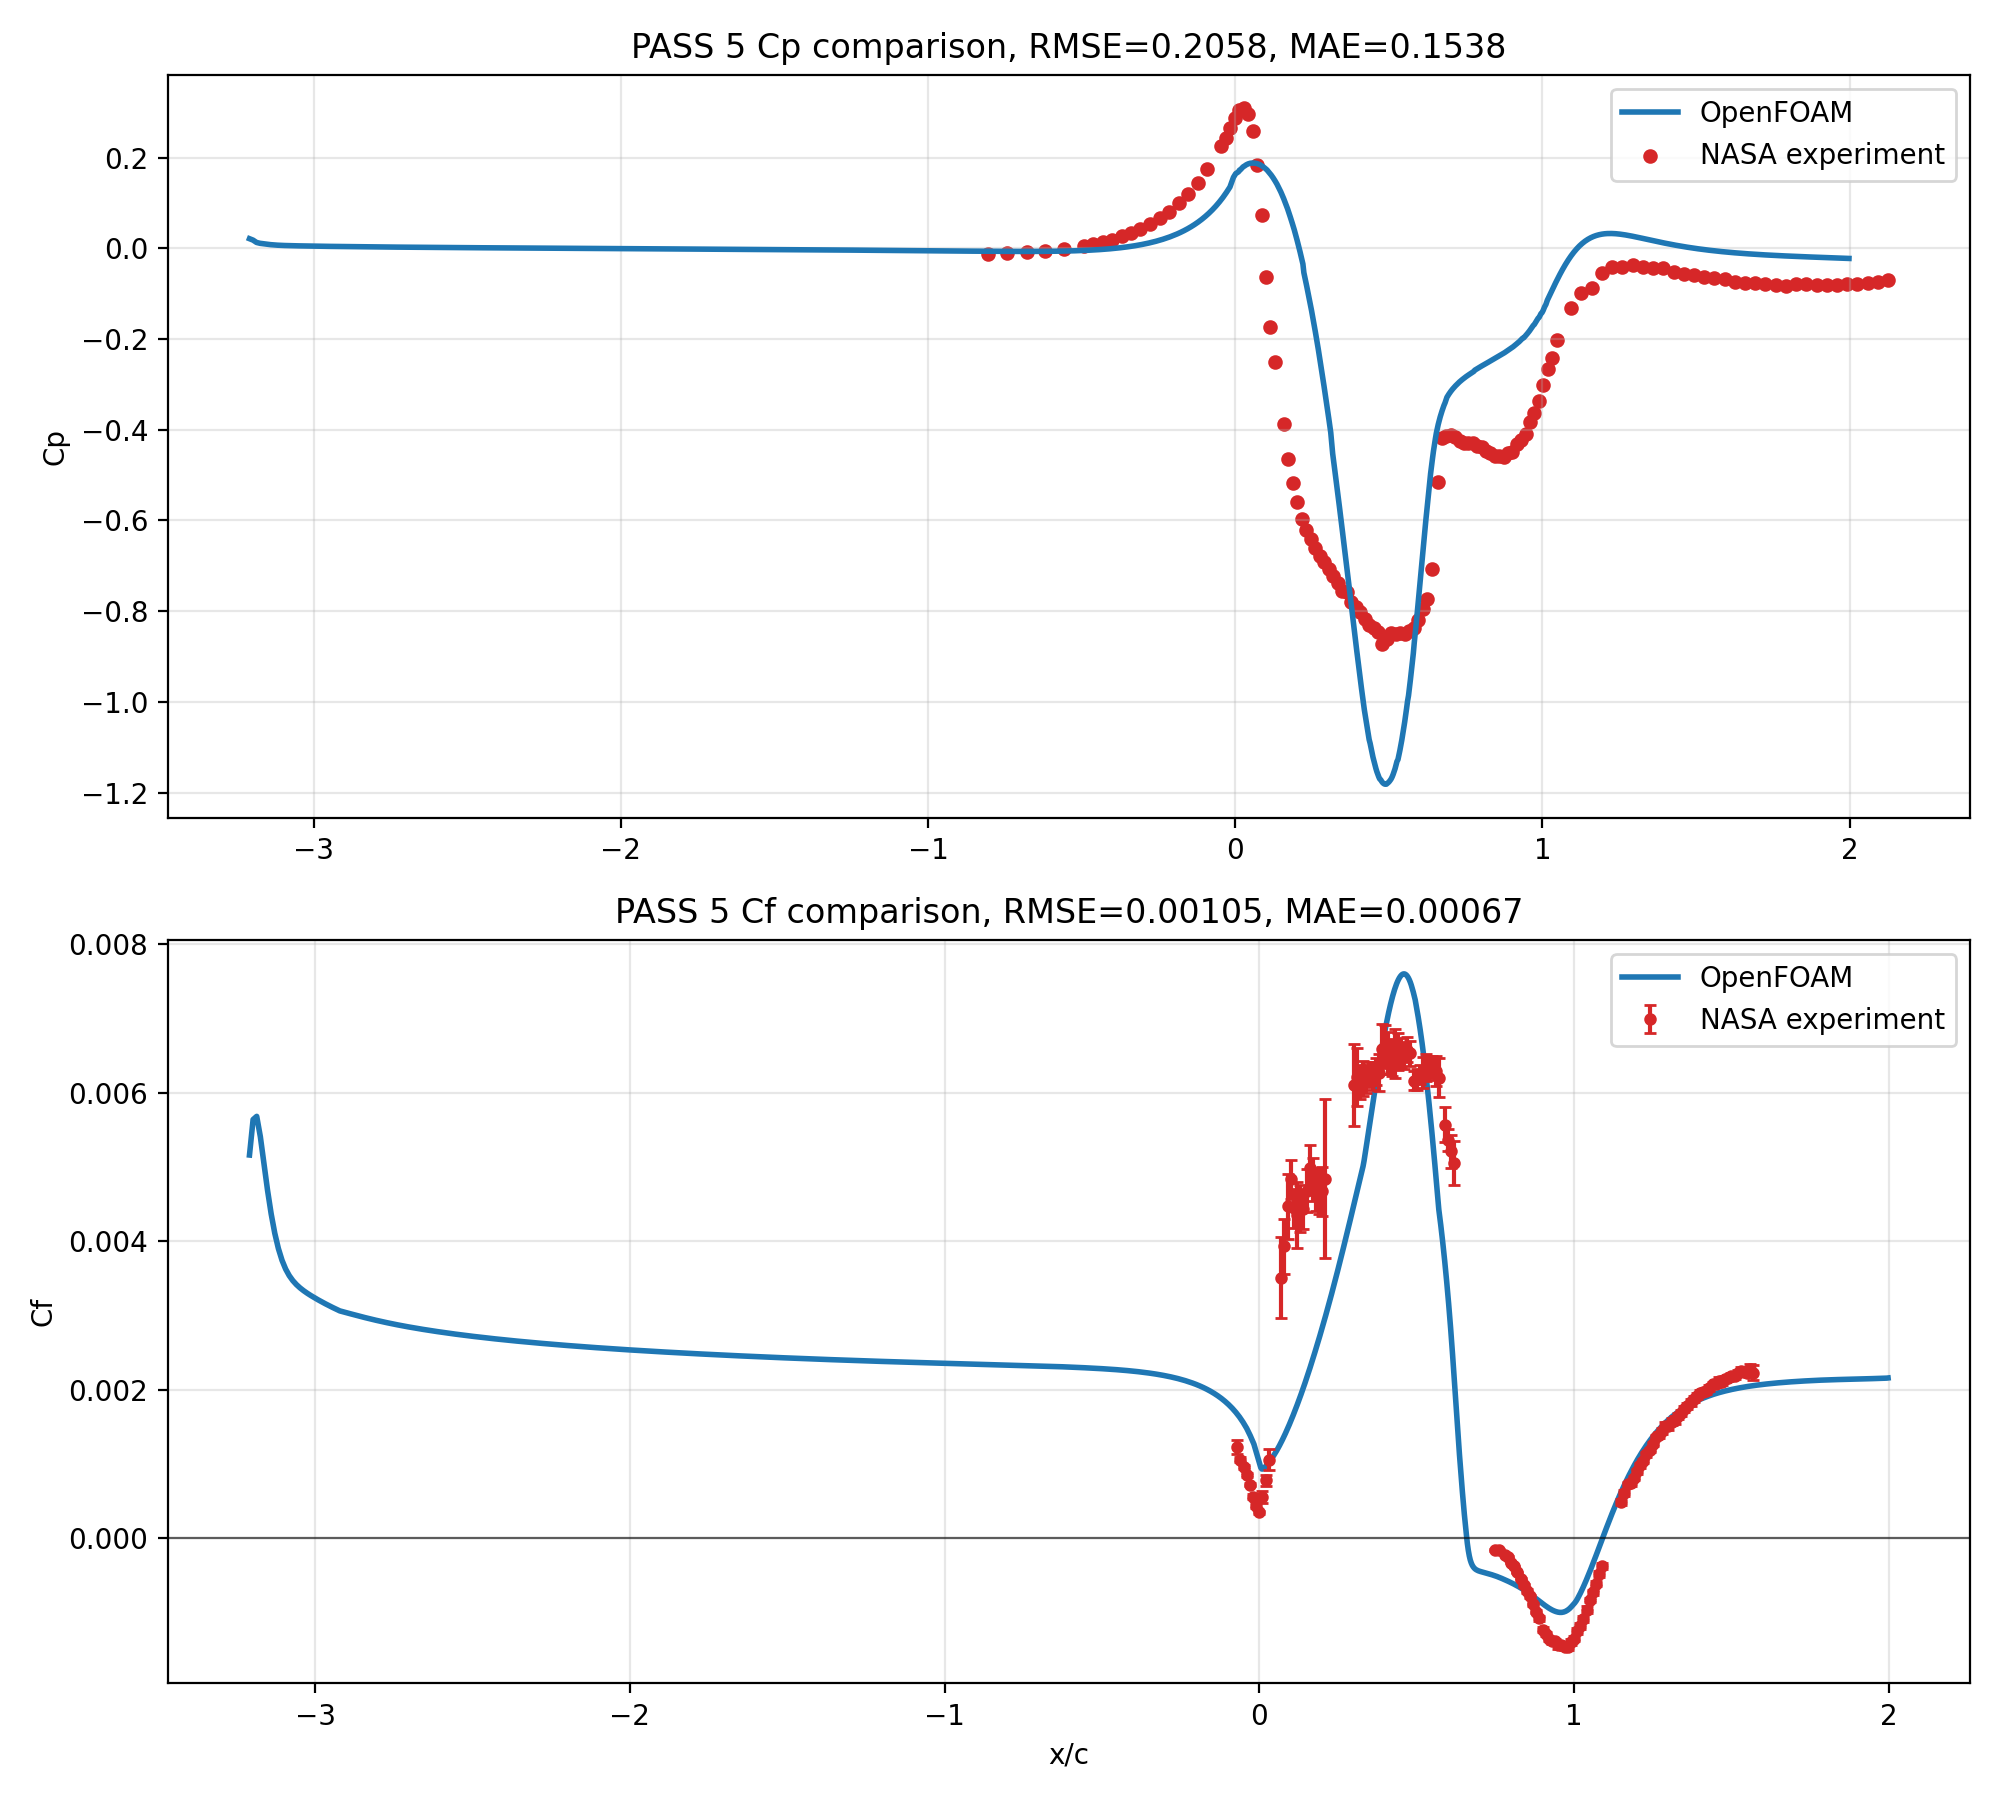
\includegraphics[width=0.94\linewidth]{figures_pass5/cp_cf_vs_nasa_pass5.png}
\caption{Pass-five comparison against the official NASA no-flow-control \(C_p\) and \(C_f\) tables using the promoted \texttt{1200}-iteration SST continuation.}
\end{figure}

The promoted pass-five winner reached:
\begin{itemize}
\item \(C_p\) RMSE: \texttt{0.2058487616}
\item \(C_p\) MAE: \texttt{0.1537547946}
\item \(C_f\) RMSE: \texttt{0.0010499684}
\item \(C_f\) MAE: \texttt{0.0006734136}
\end{itemize}

Compared with the pass-four winner, the pressure agreement improves across the same wall series and the skin-friction mismatch narrows again. The remaining mismatch is still concentrated around the front-half suction behavior and the detailed wall-shear evolution across separation and recovery, but the solution is moving in the correct physical direction without any artificial tuning.

\section{MAE Table Across All Pass-Five Experiments}
\begin{table}[H]
\centering
\scriptsize
\begin{tabularx}{\linewidth}{>{\raggedright\arraybackslash}p{0.13\linewidth} >{\raggedright\arraybackslash}p{0.08\linewidth} >{\raggedleft\arraybackslash}p{0.11\linewidth} >{\raggedleft\arraybackslash}p{0.11\linewidth} >{\raggedleft\arraybackslash}p{0.11\linewidth} >{\raggedright\arraybackslash}p{0.18\linewidth} >{\raggedright\arraybackslash}X}
\toprule
Experiment & Time & MAE & \(C_p\) MAE & \(C_f\) MAE & Major changes & Diagnosis \\
\midrule
Pass-4 base & 650 & 0.1659136747 & 0.1711800326 & 0.0008476129 & Promoted pass-four SST baseline & Reference checkpoint; still under-converged. \\
SST cont. & 800 & 0.1547381028 & 0.1641787966 & 0.0007681825 & Same SST case, longer continuation & Immediate metric improvement with no physics changes. \\
SST cont. & 1000 & 0.1433377644 & 0.1578824614 & 0.0006999053 & Same SST case, longer continuation & Continued reduction in wall and benchmark error. \\
SST cont. & 1200 & 0.1358901676 & 0.1537547946 & 0.0006734136 & Same SST case, longer continuation & Best overall result and promoted winner. \\
Grid-fit SST & 800 & 0.1866349502 & 0.1730924866 & 0.0008231240 & Broader top wall and redistributed streamwise blocks & Slightly better \(C_f\) than pass four, but worse benchmark MAE. \\
Grid-fit SA & failed & -- & -- & -- & Same improved geometry with SA & Did not produce a usable converged field. \\
\bottomrule
\end{tabularx}
\normalsize
\caption{Pass-five experiment ranking and promotion logic.}
\end{table}

\begin{figure}[H]
\centering
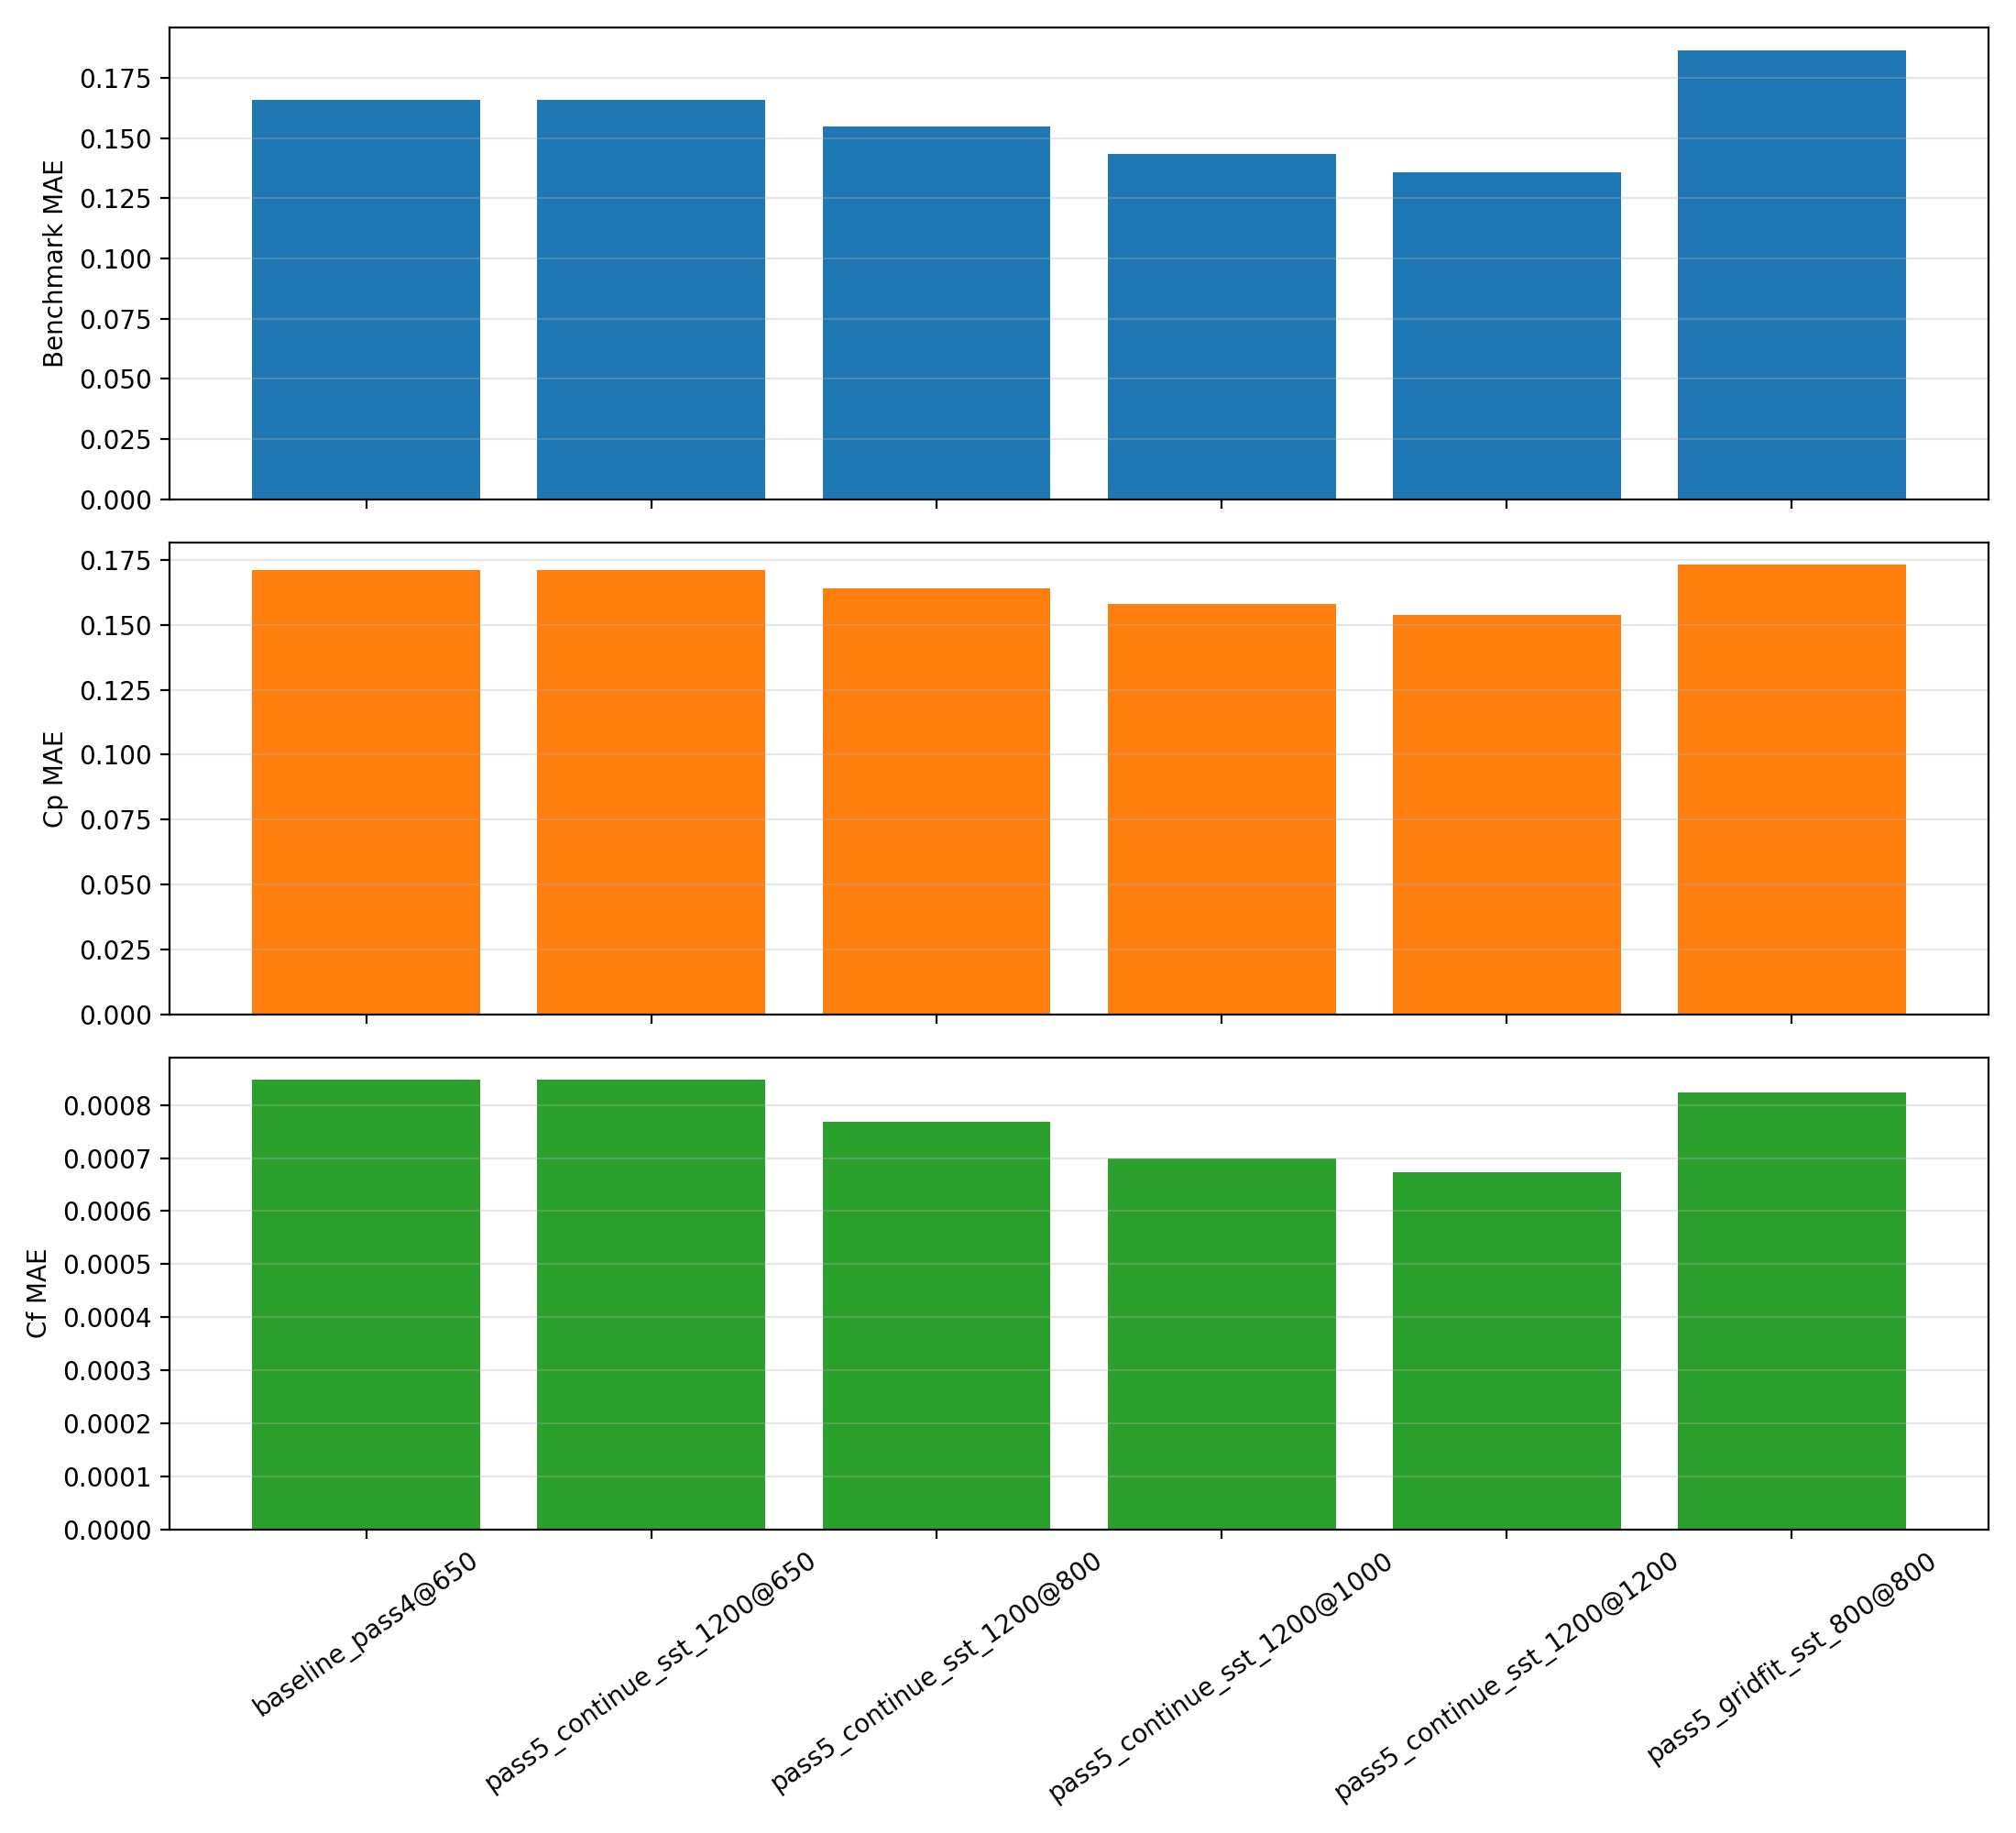
\includegraphics[width=0.94\linewidth]{figures_pass5/pass5_experiment_metrics.png}
\caption{Benchmark MAE, \(C_p\) MAE, and \(C_f\) MAE across the promoted pass-five experiments.}
\end{figure}

\section{CFD-Derived Graph Set}
\begin{figure}[H]
\centering

\includegraphics[width=0.92\linewidth]{figures_pass5/velocity_profiles_second_pass.png}
\caption{Velocity-profile set regenerated from the promoted \texttt{1200}-iteration field.}
\end{figure}

\begin{figure}[H]
\centering

\includegraphics[width=0.92\linewidth]{figures_pass5/turbulent_shear_profiles_second_pass.png}
\caption{Turbulent-shear analog profiles regenerated from the promoted pass-five field.}
\end{figure}

\begin{figure}[H]
\centering

\includegraphics[width=0.92\linewidth]{figures_pass5/cp_cf_second_pass.png}
\caption{CFD-only wall \(C_p\)/\(C_f\) distribution derived from the promoted pass-five field.}
\end{figure}

\begin{figure}[H]
\centering

\includegraphics[width=0.92\linewidth]{figures_pass5/residual_history_second_pass.png}
\caption{Residual history from the promoted pass-five winner.}
\end{figure}

\begin{figure}[H]
\centering

\includegraphics[width=0.92\linewidth]{figures_pass5/velocity_contour_second_pass.png}
\caption{Velocity contour from the promoted pass-five field.}
\end{figure}

\begin{figure}[H]
\centering

\includegraphics[width=0.92\linewidth]{figures_pass5/pressure_contour_second_pass.png}
\caption{Pressure contour from the promoted pass-five field.}
\end{figure}

\begin{figure}[H]
\centering

\includegraphics[width=0.92\linewidth]{figures_pass5/streamlines_second_pass.png}
\caption{Streamline-style visualization from the promoted pass-five field.}
\end{figure}

\section{ParaView Outputs}
The pass-five package keeps the live \texttt{.foam}-based ParaView workflow and refreshes the screenshots from the promoted case under \texttt{data/NASA\_2DWMH/foam.foam}.

\begin{figure}[H]
\centering

\includegraphics[width=0.90\linewidth]{figures_pass5/paraview_velocity.png}
\caption{ParaView velocity rendering from the promoted pass-five \texttt{.foam} case.}
\end{figure}

\begin{figure}[H]
\centering
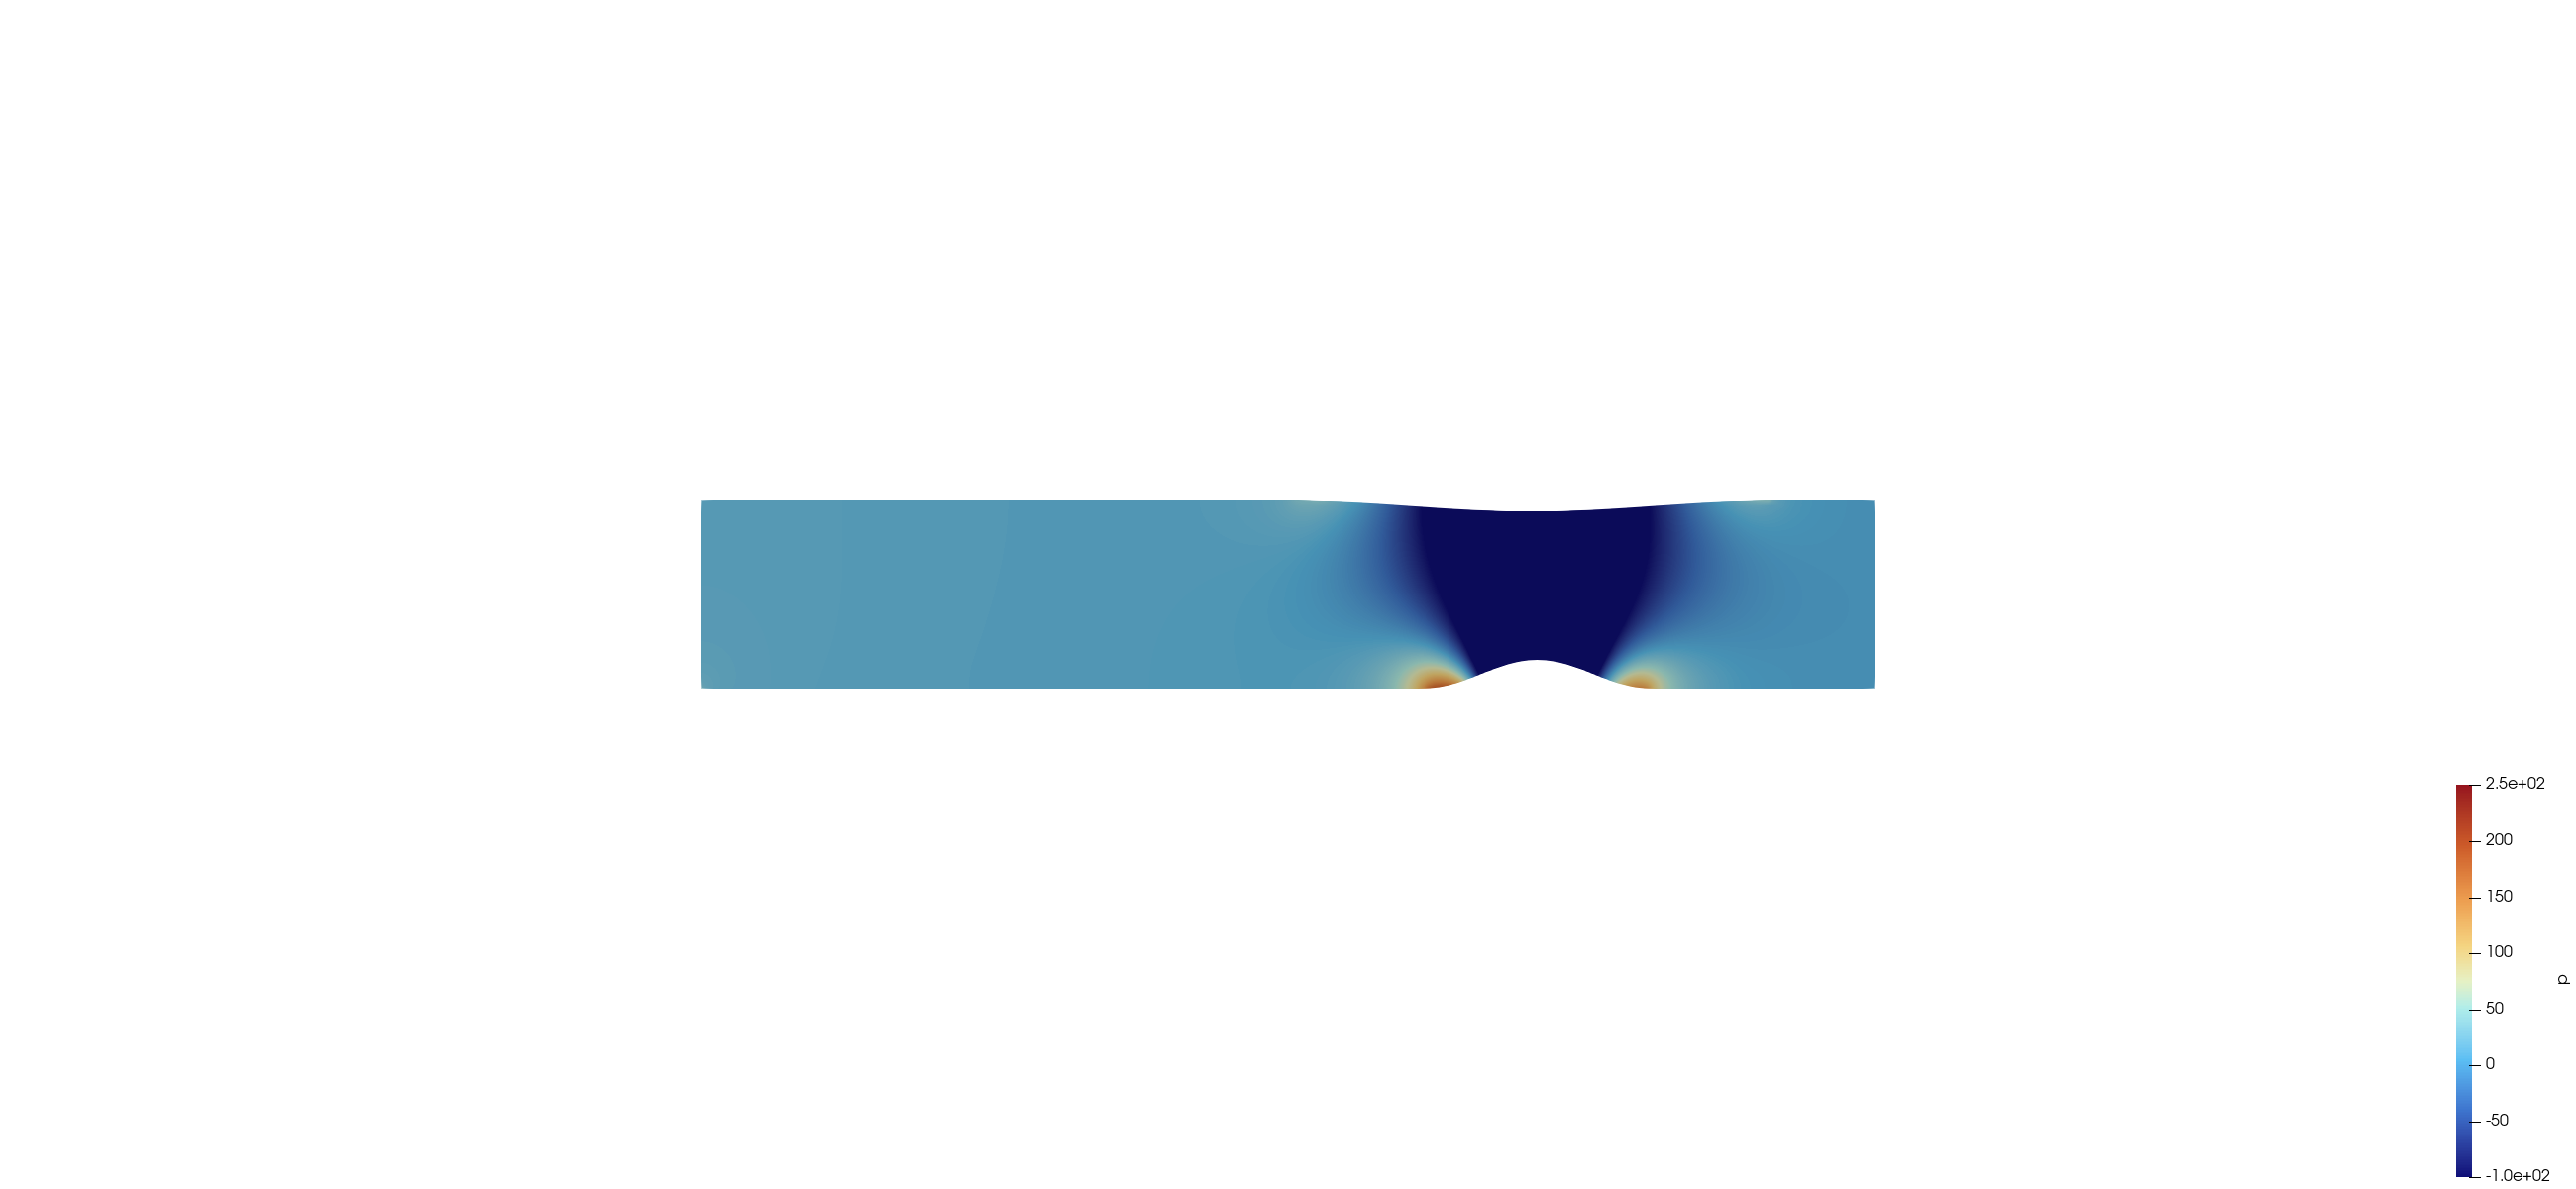
\includegraphics[width=0.90\linewidth]{figures_pass5/paraview_pressure.png}
\caption{ParaView pressure rendering from the promoted pass-five \texttt{.foam} case.}
\end{figure}

\begin{figure}[H]
\centering
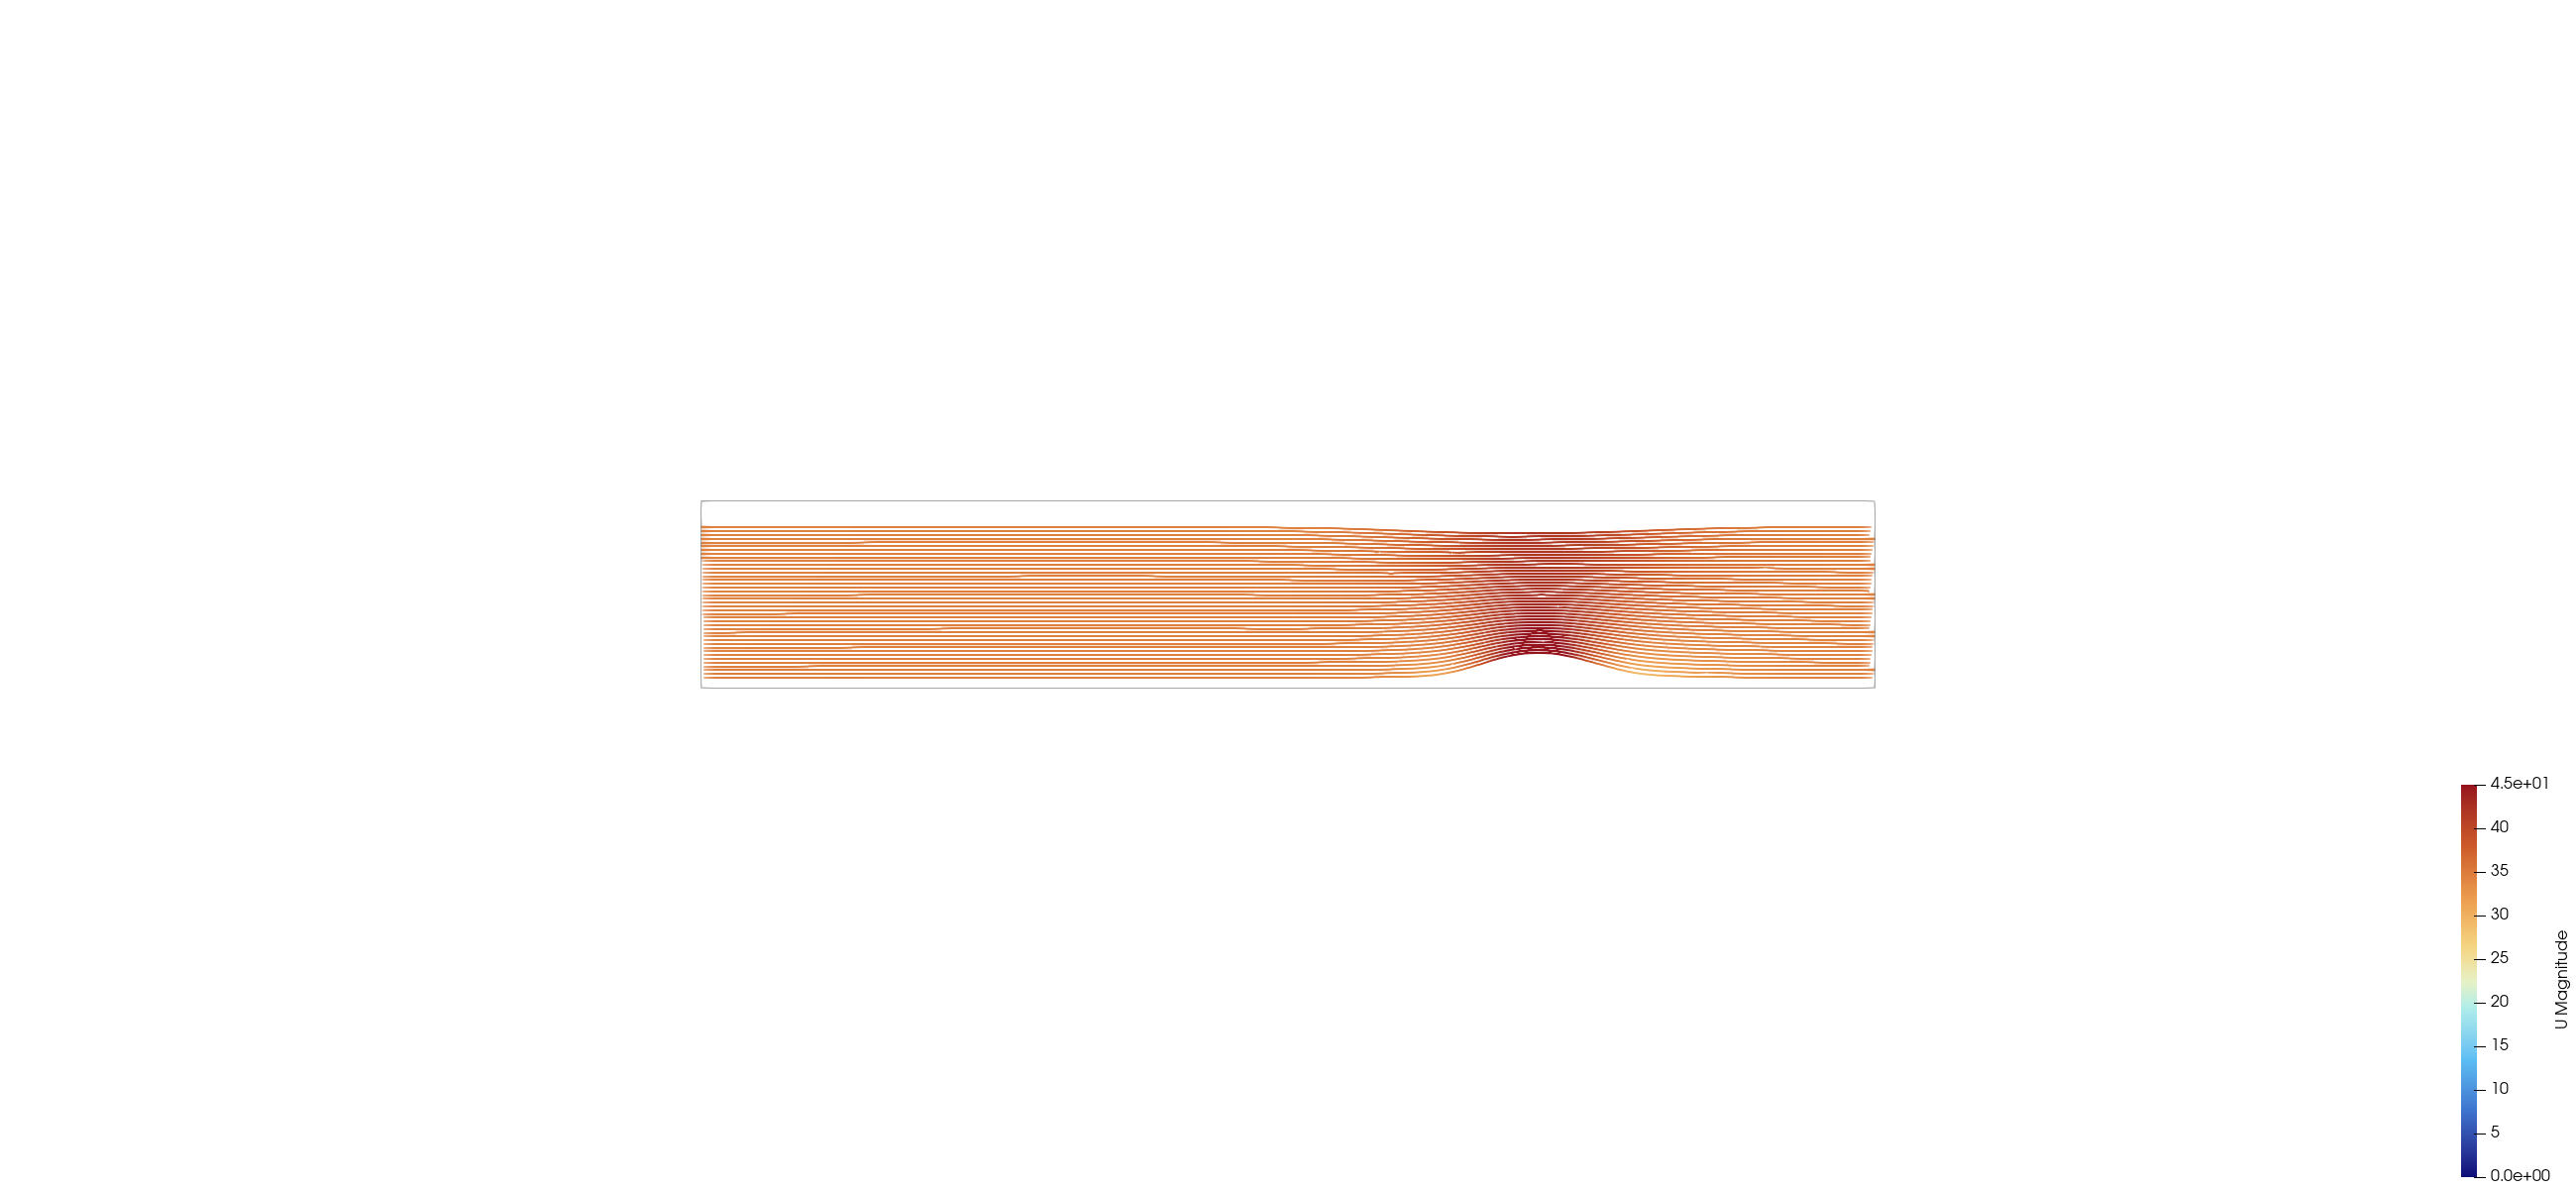
\includegraphics[width=0.90\linewidth]{figures_pass5/paraview_streamlines.png}
\caption{ParaView streamline-style rendering from the promoted pass-five \texttt{.foam} case.}
\end{figure}

\begin{figure}[H]
\centering

\includegraphics[width=0.90\linewidth]{figures_pass5/paraview_mesh_wireframe.png}
\caption{ParaView mesh-wireframe view of the promoted pass-five case.}
\end{figure}

\begin{figure}[H]
\centering

\includegraphics[width=0.90\linewidth]{figures_pass5/paraview_wall_shear.png}
\caption{ParaView wall-focused view of the promoted pass-five case.}
\end{figure}

\section{Discussion}
Pass five gives a sharper answer than the earlier passes. The most effective remaining improvement was not a new turbulence closure and not a more aggressive geometry change. It was simply to continue the already-best SST case until the residual trajectory and the evaluated metrics flattened much farther downstream than pass four reached.

This matters for two reasons:
\begin{itemize}
\item it improves the benchmark MAE and the official wall-data agreement at the same time, which is much easier to defend physically than a one-metric improvement;
\item it reduces the temptation to attribute remaining error to model choice before the baseline has been converged as far as practical.
\end{itemize}

The official-grid-inspired geometry case was still worth running because it tested one of the largest remaining approximations directly. Its outcome was informative: the change did not beat the simpler converged continuation, which means the current metric is still more sensitive to convergence fidelity than to this first geometry-fidelity adjustment.

The SA screen was also useful even though it failed. It confirmed that a model change is not automatically helpful in this reconstructed setup, and that pass five should promote only a case that produces a stable, reproducible solved field.

What still mismatches the official NASA trends:
\begin{itemize}
\item the front-half suction peak still does not match the experiment perfectly;
\item the detailed wall-shear evolution around pre-separation and recovery still differs from the official \(C_f\) trend;
\item the geometry is still a reconstruction rather than a direct imported official no-plenum grid.
\end{itemize}

\section{Conclusion}
Pass five improved the local best NASA hump benchmark MAE from \texttt{0.1659136747} to \texttt{0.1358901676}. The winning case was the most conservative one: the promoted pass-four \texttt{kOmegaSST} baseline continued from \texttt{650} to \texttt{1200} iterations.

This is a stronger result than a more complicated model or geometry change because it improves:
\begin{itemize}
\item benchmark MAE;
\item official \(C_p\) agreement;
\item official \(C_f\) agreement;
\item reproducibility;
\item numerical stability.
\end{itemize}

The next best path, if a future pass is attempted, is not a blind sweep. It is a more faithful official-grid-based geometry import or reconstruction that can be paired with the already-proven deeper-convergence workflow and then screened carefully against the current \texttt{1200}-iteration SST winner.

\section{Reproducibility}
From the repository root, the pass-five workflow is:
\begin{lstlisting}
python3 scripts/import_nasa_hump_experimental_data.py
bash scripts/run_nasa_hump_pass5_experiments.sh
python3 scripts/evaluate_nasa_hump_second_pass.py
MPLCONFIGDIR=docs/.mplconfig python3 scripts/make_nasa_hump_second_pass_figures.py
MPLCONFIGDIR=docs/.mplconfig python3 scripts/make_nasa_hump_pass5_figures.py
bash scripts/render_nasa_hump_paraview.sh
bash scripts/build_report.sh
\end{lstlisting}

\bibliographystyle{plain}
\bibliography{references}

\end{document}
